% ICLR 2027 submission — Introspective Verification
% Uses the official ICLR style (iclr2027_conference.sty/.bst + fancyhdr.sty).
\documentclass{article}
\usepackage{iclr2027_conference,times}

% Math
\usepackage{amsmath,amssymb,amsfonts,amsthm,mathtools}

% Typography
\usepackage[utf8]{inputenc}
\usepackage[T1]{fontenc}
\usepackage{hyperref}
\usepackage{url}
\usepackage{booktabs}
\usepackage{nicefrac}
\usepackage{microtype}
\usepackage{xcolor}
\usepackage{graphicx}
\usepackage{subcaption}
\usepackage{multirow}
\usepackage{rotating}
\usepackage{algorithm}
\usepackage{algorithmic}
\usepackage{pgfplots}
\pgfplotsset{compat=1.16}
\usepgfplotslibrary{groupplots}
\usepackage[most]{tcolorbox}
\usepackage{tabularx}
\newcommand{\vgood}{\textcolor{green!50!black}{\checkmark}}
\newcommand{\vbad}{\textcolor{red!75!black}{\ensuremath{\times}}}

% cleveref must be loaded AFTER hyperref
\usepackage[capitalize,noabbrev]{cleveref}

% Theorems
\theoremstyle{plain}
\newtheorem{theorem}{Theorem}[section]
\newtheorem{proposition}[theorem]{Proposition}
\newtheorem{lemma}[theorem]{Lemma}
\newtheorem{corollary}[theorem]{Corollary}
\theoremstyle{definition}
\newtheorem{definition}[theorem]{Definition}
\newtheorem{assumption}[theorem]{Assumption}
\theoremstyle{remark}
\newtheorem{remark}[theorem]{Remark}
\crefname{assumption}{Assumption}{Assumptions}
\Crefname{assumption}{Assumption}{Assumptions}

% Shared math commands
\input{math_commands}

% === ANONYMOUS SUBMISSION ===
% Uncomment \iclrfinalcopy for the camera-ready version.
% \iclrfinalcopy

\title{Introspective Verification: Reading Step Correctness at Intermediate Depth}

\author{Anonymous authors\\Paper under double-blind review}

\newcommand{\fix}{\marginpar{FIX}}
\newcommand{\new}{\marginpar{NEW}}

\begin{document}

\maketitle

\begin{abstract}
% Abstract for the Introspective Verification paper.
% Style: plain, direct; no em-dashes; minimal colons/quotes; no anthropomorphic verbs.
% Numbers verified against GenPRM (arXiv:2504.00891) Table 1 and ProcessBench.
% Citation keys used elsewhere: processbench, genprm, mathshepherd, azaria2023internal.

Process reward models score the correctness of individual reasoning steps, and the most accurate models today produce this score by generating a natural language critique and, in some systems, by executing code before a verdict. This procedure is accurate but expensive, because every step requires autoregressive decoding and an external interpreter. We ask whether the same judgment is available without generation. We find that step correctness is already encoded in the hidden states of the verifier backbone, and that an intermediate layer near seventy percent of the depth separates correct from incorrect steps more strongly than the final layer when probed. We call the resulting operation introspection: the verdict for a step is decoded from the backbone's own intermediate representation instead of being generated. This probed signal is stronger at the intermediate layer because the final state is optimized to emit the verdict token while an earlier state is formed before that token is produced. Once a readout is trained the final layer becomes the stronger single view, and the residual head combines the two. We build an introspective verdict head (LVH), a small residual classifier that combines one intermediate layer with the final layer and returns a per step reward in a single forward pass, with no generation and no code execution. The backbone is adapted with LoRA on step labels, and both training and inference run on a single V100 at the 1.5B and the 7B scale. On ProcessBench with a 1.5B backbone, the head reaches 58.1 mean F1. This exceeds most process reward models on the same benchmark, including trained process reward models at 7B and 14B scale, and it approaches the 61.9 of GPT-4o, a much larger general model used as a critic without a process reward model, while processing about one quarter of the tokens of a single generative pass. The head is also complementary to generative verifiers. Combined with a 7B generative model in logit space, on 120 case slices and with an unsupervised per domain calibration, it raises mean F1 from 76.8 to 77.4 without lowering any subset.

\end{abstract}

% Introduction for the Introspective Verification paper.
% Style: plain, direct; no em-dashes; minimal colons/quotes; no anthropomorphic verbs;
% attention to sentence-to-sentence logic. Citation keys are placeholders to be
% resolved against DBLP/CrossRef: processbench (ProcessBench), genprm (GenPRM),
% mathshepherd (Math-Shepherd), azaria2023internal (internal-state probing).

\section{Introduction}
\label{sec:intro}

Reliable multi step reasoning depends on the ability to tell which step first goes wrong, and process reward models supply this signal by scoring each step rather than only the final answer \citep{cobbe2021gsm8k, uesato2022solving, lightman2023lets}. Such scores drive selection and search at test time and shape rewards during training \citep{wang2022selfconsistency, snell2024scaling}. The labels that train these models are costly. They come from human annotation \citep{lightman2023lets}, from Monte Carlo rollouts that estimate whether a step still leads to the correct answer \citep{wang2023mathshepherd}, or from consensus filtering between rollouts and a language model judge \citep{zhang2025lessons}. ProcessBench made step level accuracy directly comparable across methods \citep{zheng2024processbench}, and a recent survey maps the fast growth of the area \citep{zheng2025survey}.

\begin{figure}[t]
  \centering
  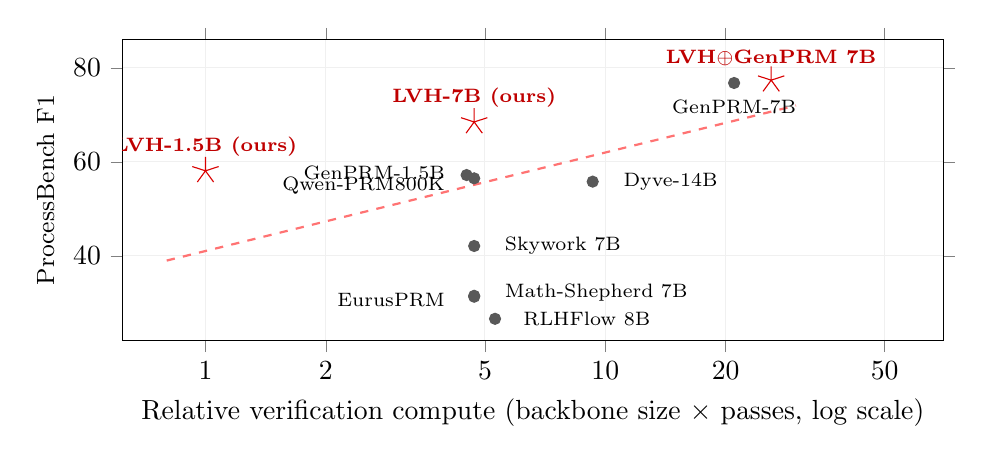
\begin{tikzpicture}
    \begin{axis}[
      width=0.99\linewidth, height=5.4cm,
      xmode=log, log basis x=10,
      xlabel={Relative verification compute (backbone size $\times$ passes, log scale)},
      ylabel={ProcessBench F1}, ylabel style={font=\small},
      xmin=0.62, xmax=70, ymin=22, ymax=86,
      xtick={1,2,5,10,20,50}, xticklabels={1,2,5,10,20,50},
      grid=both, grid style={gray!12}, tick align=outside,
    ]
    % trend guide through the trained baselines
    \addplot[dashed, red!55, thick, forget plot] coordinates {(0.8,39) (30,72)};
    % baseline process reward models
    \addplot[only marks, mark=*, mark size=2pt, gray!70!black, forget plot]
      coordinates {(4.5,57.2) (4.7,56.5) (9.3,55.8) (4.7,42.1) (4.7,31.5) (4.7,31.3) (5.3,26.6) (21,76.8)};
    % ours (three red stars: LVH-1.5B, LVH-7B, and the 7B fusion)
    \addplot[only marks, mark=star, mark size=5pt, red!85!black, forget plot]
      coordinates {(1,58.1) (4.7,68.5) (26,77.4)};
    % our method labels (above the stars, in clear space)
    \node[anchor=south, font=\scriptsize\bfseries, red!75!black] at (axis cs:1,59.0) {LVH-1.5B (ours)};
    \node[anchor=south, font=\scriptsize\bfseries, red!75!black] at (axis cs:4.7,69.6) {LVH-7B (ours)};
    \node[anchor=south, font=\scriptsize\bfseries, red!75!black] at (axis cs:26,78.3) {LVH$\oplus$GenPRM 7B};
    % left cluster: labels extend left into empty space
    \node[anchor=east, font=\scriptsize] at (axis cs:4.2,57.6) {GenPRM-1.5B};
    \node[anchor=east, font=\scriptsize] at (axis cs:4.2,54.9) {Qwen-PRM800K};
    \node[anchor=east, font=\scriptsize] at (axis cs:4.2,30.6) {EurusPRM};
    % right side: labels extend right into empty space
    \node[anchor=west, font=\scriptsize] at (axis cs:10.5,55.8) {Dyve-14B};
    \node[anchor=west, font=\scriptsize] at (axis cs:5.3,42.1) {Skywork 7B};
    \node[anchor=west, font=\scriptsize] at (axis cs:5.3,32.2) {Math-Shepherd 7B};
    \node[anchor=west, font=\scriptsize] at (axis cs:5.9,26.6) {RLHFlow 8B};
    \node[anchor=north, font=\scriptsize] at (axis cs:21,75.3) {GenPRM-7B};
    \end{axis}
  \end{tikzpicture}
  \caption{Introspective verification is compute efficient. Mean ProcessBench localization F1 against the relative compute of one verification, taken as the backbone size times the number of forward passes on a log scale, a rough proxy (the token and wall clock accounting is in \Cref{sec:exp-compute}). The introspective head (stars) sits above the trend of trained process reward models at both scales. From a single forward pass and no generation, LVH-1.5B beats the classification models outright and matches a PRM800K model at 7B and Dyve at 14B, and LVH-7B reaches 68.5 above every same cost baseline. Fused with a generative verifier it passes GenPRM-7B at a small added cost.}
  \label{fig:teaser}
\end{figure}

Two families dominate, and each has a clear limitation. Classification models attach a scalar head to the final layer representation and score a step in one forward pass. They are cheap, but they trail stronger verifiers, in particular on proof heavy problems where the answer is not a single number \citep{zheng2024processbench, zhang2025lessons}, which has motivated label efficient variants that still read from the final layer \citep{yuan2024free, sun2025freeprm}. Generative models close the accuracy gap by writing a critique of each step, and some also generate and run code before a verdict \citep{zhang2024genrm, zhao2025genprm, xiong2025stepwiser, khalifa2025thinkprm}. This accuracy is expensive, because it turns one verdict into a long decoded critique, an interpreter call, and often several samples for majority voting \citep{snell2024scaling}. Adaptive routing lowers the average cost but keeps generation for the hard steps \citep{zhong2025dyve}.

A separate line of evidence points to a cheaper source of the same judgment. A model's hidden states already encode whether its output is correct, which linear probes recover for factual statements and for answer accuracy \citep{azaria2023internal, kadavath2022language, burns2022discovering, marks2023geometry, orgad2024llms, liu2024universal}. Recent work turns these internal signals into rewards for Best of N selection \citep{guo2025mining}, aligns hidden states to improve reinforcement learning \citep{wang2026rightmakesmight}, steers a verifier through its latent representations \citep{zhou2026hidden, hsu2026refine}, and reads step correctness from a frozen backbone \citep{ni2025reprobe}. This evidence has been used mostly for answer level truthfulness, for selection, or for steering. Whether a discriminative read of the hidden states can match a generative process reward model on step level verification, at a fraction of its cost, has not been shown.

We show that this read is possible and competitive. A linear probe on a single intermediate layer of a frozen backbone separates correct from incorrect steps well above chance, and the signal is strongest near seventy percent of the depth rather than at the final layer. We call this operation introspection. The verdict for a step is decoded from the backbone's own intermediate representation, instead of being generated as a critique. This probed signal is stronger at the intermediate layer than at the final layer for a structural reason. The final state is optimized to emit the surface verdict token, so it follows the form of the answer and can be misled by a fluent but wrong step. An earlier state is formed before that token is produced, and it aligns more closely with whether the step follows from its premises. This is a statement about the raw separability of the two layers; once a readout is trained the final layer becomes the stronger single view, and our head combines the two (\Cref{sec:exp-ablation}). The final layer corresponds to what the model would state, while the intermediate layer corresponds to the assessment present before the statement.

Based on this finding, we build an introspective verdict head. The head sums two small readouts, one on an intermediate layer and one on the final layer, and returns a per step reward in a single forward pass. The two readouts and a LoRA adaptation of the backbone are trained on step level correctness labels. Inference uses one forward pass, with no decoding and no code execution, so a solution with $k$ steps is scored at the cost of reading it once. Training fits on a single V100 in a few hours, at the 1.5B scale and at the 7B scale, since a gradient-checkpointed backbone and two small heads stay within one device.

The residual form combines two complementary readouts. Once the backbone is trained, the intermediate layer readout alone is the weaker single view, and the final layer readout alone is strong on easier problems but weaker on proof heavy ones. The sum of the two matches the stronger single readout in mean F1 and improves the proof heavy subsets above either readout alone, so it adds accuracy where accuracy is scarce without giving up accuracy elsewhere.

We evaluate on ProcessBench. With a 1.5B backbone, the introspective head reaches 58.1 mean F1 from a single forward pass (\Cref{fig:teaser}). This exceeds most process reward models evaluated on the benchmark, including trained process reward models such as Math-Shepherd, RLHFlow, Skywork, EurusPRM, and a PRM800K model at 7B to 8B scale, and Dyve at 14B, and it exceeds a generative process reward model of the same 1.5B size. The score approaches the 61.9 of GPT-4o, a much larger general model used as a critic without a process reward model. The cost gap is large. One generative pass of the same size model generates about three times as many tokens as the head reads, so introspection uses about one quarter of the token compute of a single pass, with no autoregressive decoding and no code execution. The two signals are also complementary. A logit space combination of introspection with a generative verifier, with weights fixed on a held out set, improves mean F1 by 5.4 points over the generative verifier alone. At 7B, where the introspective head is again trained on a single V100, the generative verifier is stronger and introspection alone no longer matches it, which marks the regime where generation earns its cost. An unsupervised per domain calibration closes most of the remaining gap, and on 120 case slices the combination raises mean F1 from 76.8 to 77.4 without lowering any subset.

Our contributions are the following.
\begin{itemize}
  \item We identify introspection as a mechanism for process verification. Step correctness is decodable by a probe on the intermediate hidden states of a verifier backbone, where the intermediate layer carries a stronger signal than the final layer.
  \item We build an introspective verdict head, abbreviated LVH, a residual classifier over an intermediate and a final layer that produces per step rewards in one forward pass, trained with LoRA on step labels within a few hours on a single V100, at both the 1.5B and the 7B scale.
  \item On ProcessBench at 1.5B, the head exceeds most trained process reward models on the benchmark, including models at 7B and 14B scale, from a single forward pass that costs about one quarter of one generative pass, and it approaches GPT-4o, which uses no process reward model.
  \item A fixed combination of introspection with a generative verifier improves the generative verifier itself. It adds 5.4 mean F1 at 1.5B, and at 7B, on 120 case slices and with an unsupervised per domain calibration, it raises mean F1 from 76.8 to 77.4 without lowering any subset. We also characterize when introspection is sufficient and when generation is worth its cost.
\end{itemize}

The remaining sections define the head and its training, report the ProcessBench results and the fusion study, and analyze the layer choice and the failure cases.

% Related Work for the Introspective Verification paper.
% Style: plain, direct; no em-dashes; minimal colons/quotes; no anthropomorphic verbs.

\section{Related Work}
\label{sec:related}

\paragraph{Process reward models.}
Outcome verifiers score a full solution and improve selection over a base policy \citep{cobbe2021gsm8k}, and process reward models extend this to the step level, which gives denser feedback and better error attribution \citep{uesato2022solving, lightman2023lets}. Step labels come from human annotation \citep{lightman2023lets}, from Monte Carlo rollouts that estimate whether a step still leads to the correct answer \citep{wang2023mathshepherd}, or from consensus filtering between rollouts and a language-model judge \citep{zhang2025lessons}. ProcessBench standardized step-level evaluation and reports that most classification process reward models trail strong critic models on proof-heavy subsets \citep{zheng2024processbench}, a recent survey organizes the area \citep{zheng2025survey}, and later work extends step-level verification to structured and safety-critical reasoning \citep{pronesti2026verifiable}. These models attach a trained scalar head to the final-layer representation. Our verifier keeps a discriminative head but reads the verdict from an intermediate layer, and combines it with the final layer through a residual.

\paragraph{Generative and code-augmented verification.}
The most accurate recent verifiers produce the score by generation. A model writes a critique of the step as next-token prediction \citep{zhang2024genrm}, reasons about the step before judging it \citep{xiong2025stepwiser}, and in some systems generates and runs code before the verdict \citep{zhao2025genprm}. This accuracy comes at a cost that grows with the length of the generated critique and with the number of samples used for majority voting \citep{snell2024scaling, zhao2025genprm}. Dyve reduces the average cost by routing easy steps to a fast check and hard steps to slow generation \citep{zhong2025dyve}. Introspection removes the generation and keeps a single forward pass. It is complementary to these verifiers, and a fixed combination improves a strong generative model on every ProcessBench subset.

\paragraph{Label-efficient and shared-backbone reward models.}
Several methods lower the cost of building a process reward model. Implicit process rewards are read off an outcome-trained model through a log-ratio parameterization \citep{yuan2024free}, FreePRM pseudo-labels steps from final-answer correctness \citep{sun2025freeprm}, and ensemble prompting with reverse verification produces domain-agnostic labels \citep{tan2025aurora}. MetaStone-S1 shares the policy backbone and adds a small self-supervised scoring head for step evaluation \citep{wang2025metastone}. These designs reduce label or parameter cost, yet the score is still taken from the final representation or from generation. Our head reads an intermediate layer, and the readout depth is selected automatically rather than fixed.

\paragraph{Reading correctness from hidden states.}
Hidden states carry information about whether a model's own output is correct, which linear probes recover for factual statements \citep{azaria2023internal, kadavath2022language, burns2022discovering, marks2023geometry}, and steering along these directions changes truthfulness \citep{li2023inference}. Answer correctness and hallucination are predictable from internal states, sometimes before the answer is produced \citep{orgad2024llms, liu2024universal, cencerrado2025noanswer}. Closest to our work, hidden-state signals have been turned into rewards for Best-of-N sampling \citep{guo2025mining} and into a lightweight step verifier that probes a frozen backbone \citep{ni2025reprobe}. That line uses frozen representations and targets answer-level truthfulness or Best-of-N selection. We address step-level process verification on ProcessBench, adapt the backbone with LoRA so the representation itself improves on proof domains, combine an intermediate and a final layer, and reach the accuracy of generative process reward models at a fraction of the compute.

\paragraph{Layer-wise representations, probing, and adaptation.}
Linear classifiers on hidden states are a standard tool for locating information across depth \citep{alain2016understanding}, and lenses map intermediate states to output distributions \citep{belrose2023eliciting}. This work reports that task-relevant structure is often most decodable in intermediate layers rather than the final layer, which motivates our readout depth. Our verdict head is trained with a parameter-efficient adaptation of the backbone \citep{hu2021lora}, and the chosen depth is produced by the model's own measurement rather than set by hand. Test-time verification and self-consistency use such verifiers to select among sampled solutions \citep{wang2022selfconsistency}.

% Method section for the Introspective Verification paper.
% Style: plain, direct; no em-dashes; minimal colons/quotes; no anthropomorphic verbs.

\section{Method}
\label{sec:method}

We describe the introspective verdict head, which reads a per step reward from the backbone's hidden states in a single forward pass. We fix notation (\Cref{sec:method-setup}), define the head (\Cref{sec:method-head}), explain the layer choice (\Cref{sec:method-layer}), state the training objective (\Cref{sec:method-train}), and give the inference procedure and its cost (\Cref{sec:method-infer}). An optional logit space fusion with a generative verifier is in \Cref{sec:method-fusion}.

\subsection{Setup and notation}
\label{sec:method-setup}

A problem $x$ has a candidate solution written as an ordered sequence of steps $s_1,\dots,s_k$. A process verifier assigns each step a reward $r_i \in [0,1]$, where a reward above a threshold marks the step as an error, and the first such step is the located error. ProcessBench scores this located first error against the labeled one.

The backbone is a decoder only transformer $f$ with $L$ layers. For an input token sequence it returns hidden states $h^{(0)},\dots,h^{(L)}$, where $h^{(0)}$ is the embedding and $h^{(L)}$ is the final layer. We write $h_i^{(\ell)} \in \R^{d}$ for the hidden state at layer $\ell$ at the last token of step $s_i$, that is the token that ends the step in the concatenation $x, s_1, \dots, s_k$. Because attention is causal, this last token has attended to all of $x$ and $s_1,\dots,s_i$, so its hidden state is a natural summary of the step in the context that precedes it. Reading a per step reward from $h_i^{(\ell)}$ therefore requires no extra generation, only the states that a single pass over the solution already produces.

\subsection{The introspective verdict head}
\label{sec:method-head}

The head sums two readouts, one on the final layer and one on an intermediate layer $\ell^\star$,
\begin{equation}
  r_i \;=\; \sigma\!\big(\underbrace{\vw^\top h_i^{(L)}}_{\text{stated verdict}} \;+\; \underbrace{g\big(h_i^{(\ell^\star)}\big)}_{\text{latent assessment}}\big),
  \qquad
  z_i \;\triangleq\; \vw^\top h_i^{(L)} + g\big(h_i^{(\ell^\star)}\big),
  \label{eq:head}
\end{equation}
where $\vw \in \R^{d}$ is a linear map on the final layer, $g:\R^{d}\to\R$ is a two layer perceptron with a GELU nonlinearity ($\R^{d}\!\to\!\R^{m}\!\to\!\R$, with $m=512$), $\sigma$ is the logistic function, and $z_i$ is the pre sigmoid logit of the reward. The two readouts play different roles. The final layer readout follows the verbalized verdict that the backbone would emit, so it is the stated view, presentation oriented and prone to fluent but wrong steps. The intermediate readout is taken before that surface token is formed, so it is the latent view, the assessment behind the answer. Their residual sum keeps the calibration of the stated view and the discrimination of the latent view, and \Cref{fig:arch} contrasts this single pass read with a generative verifier that decodes a critique, runs code, and votes over samples.

\begin{figure}[t]
  \centering
  \IfFileExists{figures/method_arch.png}
    {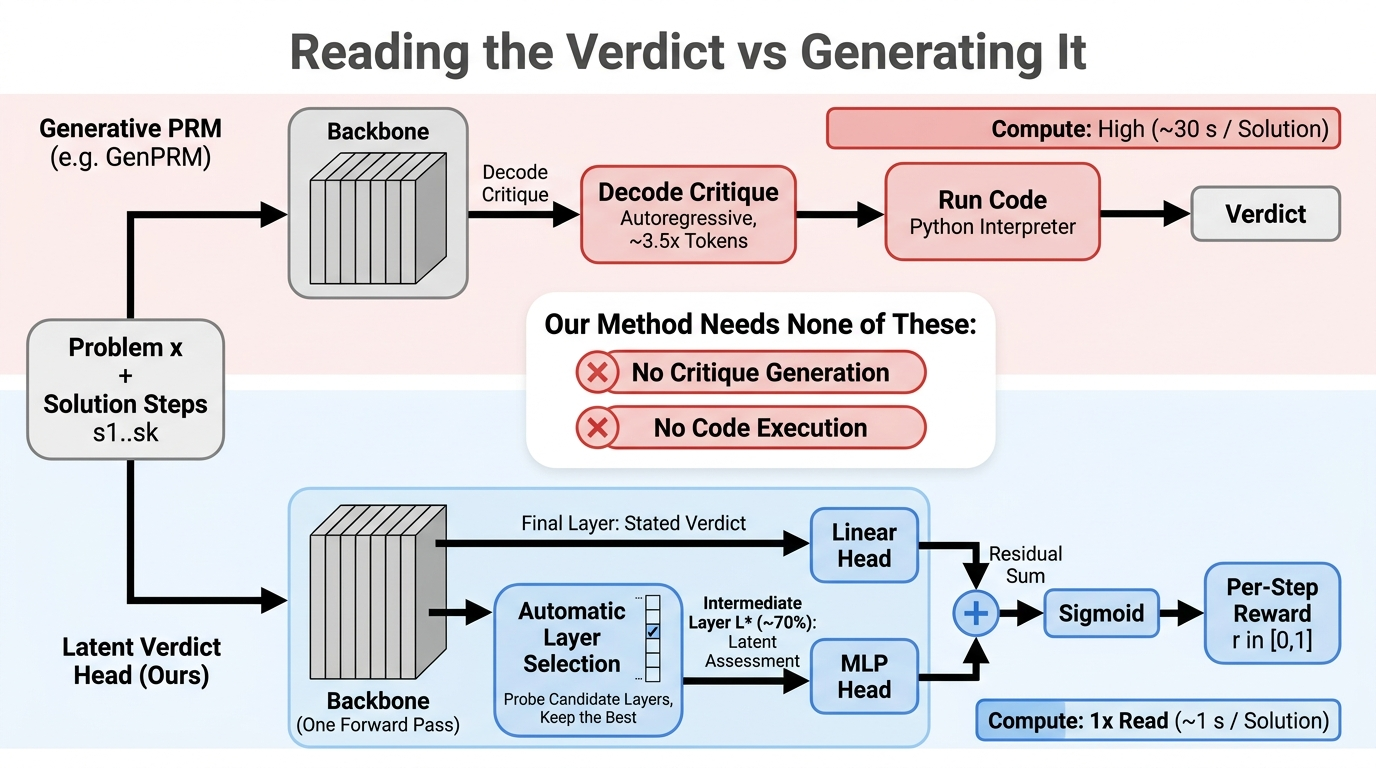
\includegraphics[width=0.9\linewidth]{figures/method_arch}}
    {\fbox{\parbox[c][4.2cm][c]{0.9\linewidth}{\centering\itshape figures/method\_arch.png \\ (architecture diagram: backbone with a mid layer and final layer tap, an MLP head and a linear head summed into a per step reward, one forward pass)}}}
  \caption{Reading the verdict instead of generating it. Top: a generative process reward model decodes a natural language critique, runs code, and often votes over several samples before a verdict, which costs many decoded tokens and an interpreter call. Bottom: the introspective verdict head reads the same solution in a single forward pass, taps the final layer for the stated verdict and an intermediate layer $\ell^\star$ for the latent assessment, and sums them into a per step reward. It needs no critique generation and no code execution, at about one quarter of the token cost of a single generative pass. Both methods use the same backbone and differ only in what follows it, and the intermediate layer $\ell^\star$ is selected automatically by a probe over candidate layers (\Cref{alg:select}).}
  \label{fig:arch}
\end{figure}

\subsection{Why an intermediate layer}
\label{sec:method-layer}

We place $\ell^\star$ at about seventy percent of the depth, nine layers below the output, which a per layer probe sweep selects (\Cref{fig:layersweep}). The reason is structural. The final state is optimized to emit the surface verdict token, so it is shaped by the form of the answer and can be moved by a step that reads fluently while being wrong. A state a few layers earlier is formed before that token is produced, and it aligns more closely with whether the step follows from its premises. The final layer corresponds to what the model would state, and the intermediate layer to the assessment that is present before the statement. \Cref{sec:exp-layer} shows that step correctness is in fact most separable at this depth and weaker at the final layer.

\subsection{Automatic layer selection}
\label{sec:method-select}

We do not fix $\ell^\star$ by hand. Before training, a cheap probe selects it automatically from a small labeled set, as in \Cref{alg:select}. For each candidate layer in a set $\cC$ we take the last token hidden state of every step, fit a class balanced logistic probe on step correctness, and score the located first error on a held out split. We set $\ell^\star$ to the candidate with the highest localization F1. The procedure runs once, passes no gradient through the backbone, and reuses the same step labels as training, so it adds little cost. It reads only the backbone's own features. The candidate set $\cC$ is fixed to the eight layers one, three, five, and so on up to fifteen below the output, and the labeled set is a few hundred solutions from the training distribution. We run the selection on the 7B backbone (\Cref{sec:exp-layer}), where it returns the layer nine below the output, near seventy percent of the depth, and since both backbones have 28 layers we apply the same relative depth $\ell^\star=20$ of $28$ at 1.5B. The training below then adapts the head at the selected $\ell^\star$.

\begin{algorithm}[t]
  \caption{Automatic selection of the intermediate layer $\ell^\star$}
  \label{alg:select}
  \begin{algorithmic}[1]
    \REQUIRE candidate layers $\cC$, labeled set $\cD_{\mathrm{sel}}$ with per step labels, split into fit and held out parts, frozen backbone $f$
    \FOR{each candidate layer $\ell \in \cC$}
      \STATE $X_\ell \leftarrow$ last token hidden states at layer $\ell$ for all steps in the fit part
      \STATE fit a class balanced logistic probe $p_\ell$ on $(X_\ell, y)$
      \STATE $F_\ell \leftarrow$ localization F1 of $p_\ell$ on the held out part
    \ENDFOR
    \RETURN $\ell^\star = \argmax_{\ell \in \cC} F_\ell$
  \end{algorithmic}
\end{algorithm}

\subsection{Training}
\label{sec:method-train}

We adapt the backbone with LoRA \citep{hu2021lora} of rank $16$ and scaling $32$ on the query, key, value, and output projections, and train the LoRA parameters and the two heads jointly. The rest of the backbone is frozen, and gradient checkpointing keeps the backbone and the heads within a single V100 class device at both the 1.5B and the 7B scale. Supervision is a set of step level labels $\cD=\{(x, s_{1:k}, y_{1:k})\}$ with $y_i\in\{0,1\}$, where $y_i=1$ marks an incorrect step. We minimize a class balanced binary cross entropy on the step logits of \Cref{eq:head},
\begin{equation}
  \cL \;=\; \sum_{(x,s_{1:k},y_{1:k})\in\cD}\ \sum_{i=1}^{k}\ \mathrm{BCE}\big(z_i,\, y_i\big),
  \qquad
  \text{positive weight } \frac{1-p}{p},
  \label{eq:loss}
\end{equation}
where $p$ is the fraction of error steps in $\cD$, which offsets the imbalance of rare errors. The labels come from the step level annotations released with GenPRM \citep{zhao2025genprm}. The method uses only these labels, not the generative model that produced them.

\begin{algorithm}[t]
  \caption{Introspective scoring of a $k$ step solution (inference)}
  \label{alg:score}
  \begin{algorithmic}[1]
    \REQUIRE problem $x$, steps $s_1,\dots,s_k$, adapted backbone $f$, heads $\vw, g$, layer $\ell^\star$, threshold $\tau$
    \STATE tokenize $x, s_1, \dots, s_k$ and record the last token index $t_i$ of each step
    \STATE $H \leftarrow f(x, s_{1:k})$ \hfill // one forward pass, hidden states at all layers, no decoding
    \FOR{$i = 1$ to $k$}
      \STATE $z_i \leftarrow \vw^\top H^{(L)}_{t_i} + g\big(H^{(\ell^\star)}_{t_i}\big)$; \quad $r_i \leftarrow \sigma(z_i)$
    \ENDFOR
    \STATE $e \leftarrow \min\{\, i : r_i > \tau \,\}$, or none if no step exceeds $\tau$
    \RETURN rewards $r_{1:k}$ and located first error $e$
  \end{algorithmic}
\end{algorithm}

\subsection{Inference and cost}
\label{sec:method-infer}

Inference is one forward pass. Given the problem and its steps we run the backbone once with hidden states, gather the last token index of each step, and apply \Cref{eq:head} to obtain $r_1,\dots,r_k$, as in \Cref{alg:score}. The located first error is the first step whose reward exceeds a threshold $\tau$, and $\tau$ is fixed on a held out split. There is no autoregressive decoding and no interpreter call. The cost is a single prefill over the solution of $n$ tokens, against a generative verifier that prefills the same solution and then decodes a critique on the order of $c\,n$ tokens and runs code, one forward pass per generated token. A solution with $k$ steps is therefore scored at the cost of reading it once, and \Cref{sec:exp-compute} quantifies the gap.

\subsection{Fusion with a generative verifier}
\label{sec:method-fusion}

The introspective reward and a generative verifier read different evidence, so they can be combined. Given a generative verifier's per step correctness probability $P^{B}_i$, we form a logit space score
\begin{equation}
  \zeta_i \;=\; a\,\big(z_i - c\big) \;+\; (1-a)\,\mathrm{logit}\big(1 - P^{B}_i\big),
  \label{eq:fusion}
\end{equation}
and locate the first error at the first step with $\zeta_i$ above a bias $b$. The weight $a$ and bias $b$ are fixed on a held out split and never tuned on the evaluated subset, which keeps the combination honest. The scalar $c$ is an unsupervised per domain centering that we apply only at the 7B scale, and we explain in \Cref{app:calib} why the 7B head needs it and the 1.5B head does not. The fusion adds one forward pass to the generative pipeline, so it is close to free next to repeated decoding.

% Experiments for the Introspective Verification paper.
% Style: plain, direct; no em-dashes; minimal colons/quotes; no anthropomorphic verbs.
% Numbers: LVH / GenPRM (greedy) rows from the local runs; other ProcessBench rows
% (Math-Shepherd, RLHFlow, Skywork, EurusPRM, PRM800K, Dyve, GPT-4o, GenPRM Maj@8)
% are from GenPRM (arXiv:2504.00891) Table 1, itself built on ProcessBench.

\section{Experiments}
\label{sec:experiments}

We test one claim: a discriminative read of the backbone's hidden states matches a generative process reward model on step level verification at a fraction of its cost. We recall the operation under test, describe the protocol, and then report the 1.5B result, the fusion with a generative verifier, the behavior at 7B, and the compute accounting.

\subsection{The head under test}
\label{sec:exp-head}

We evaluate the introspective verdict head of \Cref{sec:method}, which we abbreviate LVH in the tables. It scores a step in one forward pass by summing a linear readout on the final layer and an MLP readout on an automatically selected intermediate layer $\ell^\star$ (\Cref{eq:head}), with the backbone LoRA adapted on step labels, and with no decoding and no code execution. For DeepSeek-R1-Distill-Qwen the selection returns $\ell^\star=20$ of $28$, near seventy percent of the depth, and we use this layer at both scales.

\subsection{Setup}
\label{sec:exp-setup}

\paragraph{Benchmark and metric.} We evaluate on ProcessBench \citep{zheng2024processbench}, which asks a verifier to locate the first incorrect step in a solution, or to report that every step is correct. The benchmark has four subsets of increasing difficulty, GSM8K, MATH, OlympiadBench, and OmniMATH. The metric for each subset is the localization F1, the harmonic mean of two accuracies, the accuracy on erroneous solutions where the predicted first error must match the labeled step, and the accuracy on correct solutions where the verifier must predict no error. We report the four subsets and their mean.

\paragraph{Backbones.} We use DeepSeek-R1-Distill-Qwen at the 1.5B and the 7B scale as the verifier backbone. Both have 28 transformer layers, so $\ell^\star=20$ is the same relative depth at both scales. Training and inference run on a single V100 class GPU in a few hours, in bf16 or fp16, with gradient checkpointing so the backbone and the two heads stay within one device.

\paragraph{Training labels.} Supervision is the step level Yes/No labels released with GenPRM \citep{zhao2025genprm}, which come from math model trajectories with relative progress estimation. The method uses only these labels, not the GenPRM model. We train on the order of eight thousand conversations.

\paragraph{Baselines.} We compare against the process reward models tabulated on ProcessBench and by GenPRM. These are the classification models Math-Shepherd-PRM-7B \citep{wang2023mathshepherd}, RLHFlow-PRM-8B, Skywork-PRM-7B, and EurusPRM-Stage2, the discriminative Qwen2.5-Math-7B model trained on PRM800K \citep{lightman2023lets, zhang2025lessons}, the adaptive Dyve at 14B \citep{zhong2025dyve}, and GPT-4o used as a critic without a process reward model. We also compare against GenPRM at the matching 1.5B and 7B size, in both its greedy single pass form and its eight sample majority vote form. The greedy GenPRM rows are measured in our environment with the official incremental protocol, and reproduce the released scores; the remaining external rows are from GenPRM Table 1.

\subsection{An intermediate layer carries the signal}
\label{sec:exp-layer}

Before the benchmark we locate where step correctness is decodable. We freeze the 7B backbone, take the last token hidden state of each step at eight candidate layers, and fit a balanced logistic probe on step correctness. \Cref{tab:layersweep} reports two quantities per layer, the step level separability as the area under the ROC curve, and the localization F1 of the probe. Both peak at the same place. As a probe, the intermediate layer nine below the output, at about seventy percent of the depth, is the most separable on both measures, 0.915 AUC and 44.2 F1, and separability declines toward the final layer and toward the middle of the network. In raw separability the intermediate layer, not the final layer, is where step correctness reads out most cleanly. This sweep is exactly the automatic selection of \Cref{alg:select} run on the 7B backbone, so the head reads from the layer this procedure returns rather than from a hand chosen one, and \Cref{fig:layersweep} plots the full curve.

\begin{table}[t]
  \centering
  \caption{Per layer probe separability on the frozen 7B backbone. Layer $-k$ is $k$ layers below the output; relative depth is the position among the 28 transformer layers. Step correctness is most separable, on both the step level AUC and the probe localization F1, at the intermediate layer nine below the output, near seventy percent of the depth, and separability falls off toward the final layer.}
  \label{tab:layersweep}
  \begin{tabular}{lcccccccc}
    \toprule
    Layer (from top) & $-1$ & $-3$ & $-5$ & $-7$ & $-9$ & $-11$ & $-13$ & $-15$ \\
    Relative depth & 100\% & 93\% & 86\% & 79\% & \textbf{71\%} & 64\% & 57\% & 50\% \\
    \midrule
    Step AUC        & 0.907 & 0.905 & 0.896 & 0.910 & \textbf{0.915} & 0.904 & 0.889 & 0.867 \\
    Localization F1 & 42.2 & 38.7 & 39.4 & 37.7 & \textbf{44.2} & 41.2 & 33.9 & 31.2 \\
    \bottomrule
  \end{tabular}
\end{table}

\subsection{The residual form}
\label{sec:exp-ablation}

The head reads the intermediate layer, where step correctness is most separable (\Cref{tab:layersweep}), and adds a final layer readout for calibration. \Cref{tab:ablation} trains the two readouts separately and together at the same budget to show what each contributes. A trained readout is not the same as a raw probe, and the two roles are different. The final layer readout is trained to emit the verdict itself, so as a standalone readout it is well calibrated, 58.6 mean F1, even though the final layer's raw separability is the lower of the two (\Cref{tab:layersweep}). The intermediate readout alone is discriminative but poorly calibrated, 54.4, since nothing anchors the scale of its scores. The residual head keeps the intermediate layer's discrimination and the final layer's calibration. It dominates the intermediate readout on every subset, matches the calibrated final readout in the mean, and exceeds it on the two proof heavy subsets, OlympiadBench and OmniMATH, by 1.4 and 1.2 points, where discrimination matters most. The value of the residual form is therefore not a higher mean but a redistribution of accuracy toward the harder subsets at no cost elsewhere.

\begin{table}[t]
  \centering
  \caption{Contribution of each readout at 1.5B, trained at the same full budget (8000 conversations, 15000 steps), localization F1. The final readout is trained to be the verdict, so on its own it is well calibrated; the intermediate readout is discriminative but uncalibrated; the residual head keeps both and exceeds the calibrated final readout on the two proof heavy subsets. This is a trained readout comparison and is distinct from the raw separability of \Cref{tab:layersweep}. The residual mean, 58.5, matches the headline 58.1 of \Cref{tab:pb} within run to run noise.}
  \label{tab:ablation}
  \begin{tabular}{lccccc}
    \toprule
    Trained readout & GSM8K & MATH & Olympiad & OmniMATH & Mean \\
    \midrule
    Final layer only        & \textbf{67.9} & \textbf{64.3} & 51.6 & 50.7 & \textbf{58.6} \\
    Intermediate layer only & 59.7 & 58.2 & 49.9 & 49.7 & 54.4 \\
    Residual (both)         & 65.3 & 63.8 & \textbf{53.0} & \textbf{51.9} & 58.5 \\
    \bottomrule
  \end{tabular}
\end{table}

\subsection{Introspection matches a generative verifier at 1.5B}
\label{sec:exp-main}

\Cref{tab:pb} (top panel) reports the full ProcessBench result at the 1.5B scale. The introspective head reaches 58.1 mean F1 from a single forward pass. This exceeds every classification process reward model in the table, including models at 7B and 8B scale, and it exceeds the discriminative PRM800K model at 7B and Dyve at 14B. It also exceeds the same size generative model GenPRM-1.5B in its greedy form, 58.1 against 57.2, while reading the solution once rather than decoding a critique and calling an interpreter. The score approaches the 61.9 of GPT-4o, a much larger general model used as a critic. A stronger but much costlier configuration of the generative model, eight sample majority voting, reaches 63.4; sampling and voting are orthogonal and could be applied to either verifier, so we do not treat their absence as an advantage of the head. The per subset pattern is informative. The head leads on GSM8K by a wide margin, stays close on MATH and OlympiadBench, and is weakest on OmniMATH, the proof heavy subset where a cheap ranking signal is hardest to extract.

\begin{table}[t]
  \centering
  \caption{ProcessBench localization F1. \emph{Top panel:} 1.5B scale on the full benchmark. \emph{Bottom panel:} 7B scale on 120 case slices. External rows are from ProcessBench \citep{zheng2024processbench} and GenPRM \citep{zhao2025genprm} Table 1; GenPRM greedy rows are measured in our environment with the official incremental protocol and reproduce the released scores. The introspective head (LVH) uses one forward pass, with no generation and no code execution. LVH-7B standalone uses the unsupervised per domain calibration of \Cref{sec:exp-7b}; the fusion row is the honest leave one domain out combination.}
  \label{tab:pb}
  \begin{tabular}{llccccc}
    \toprule
    & Method & GSM8K & MATH & Olympiad & OmniMATH & Mean \\
    \midrule
    \multirow{10}{*}{\rotatebox{90}{\textbf{1.5B} \; full}}
    & Math-Shepherd-PRM-7B      & 47.9 & 29.5 & 24.8 & 23.8 & 31.5 \\
    & RLHFlow-PRM-8B            & 38.8 & 33.8 & 16.9 & 16.9 & 26.6 \\
    & Skywork-PRM-7B           & 70.8 & 53.6 & 22.9 & 21.0 & 42.1 \\
    & EurusPRM-Stage2          & 47.3 & 35.7 & 21.2 & 20.9 & 31.3 \\
    & Qwen2.5-Math-7B-PRM800K  & 68.2 & 62.6 & 50.7 & 44.3 & 56.5 \\
    & Dyve-14B                 & 68.5 & 58.3 & 49.0 & 47.2 & 55.8 \\
    & GPT-4o (critic, no PRM)  & 79.2 & 63.6 & 51.4 & 53.5 & 61.9 \\
    & GenPRM-1.5B (greedy)     & 52.8 & 66.6 & 55.1 & 54.5 & 57.2 \\
    & GenPRM-1.5B (Maj@8)      & 51.3 & 74.4 & 65.3 & 62.5 & 63.4 \\
    & \textbf{LVH-1.5B (ours, one pass)} & \textbf{65.1} & 61.3 & 53.5 & 52.4 & \textbf{58.1} \\
    \midrule
    \multirow{3}{*}{\rotatebox{90}{\textbf{7B}}}
    & GenPRM-7B (greedy)       & 83.4 & 80.0 & 72.3 & 71.5 & 76.8 \\
    & LVH-7B (ours, one pass)  & 72.5 & 76.6 & 68.1 & 57.0 & 68.5 \\
    & \textbf{LVH $\oplus$ GenPRM-7B (fusion)} & \textbf{83.4} & \textbf{81.5} & \textbf{73.2} & \textbf{71.5} & \textbf{77.4} \\
    \bottomrule
  \end{tabular}
\end{table}

\subsection{Where the head succeeds and fails}
\label{sec:exp-erranalysis}

\Cref{tab:perdomain} splits the localization F1 into its parts, the accuracy on erroneous solutions and on correct ones, and on the error side the fractions where the head places the error correctly, flags the wrong step, or misses the error. The failure mode shifts with difficulty. On GSM8K the head mostly misses errors, 25.1 percent, and rarely mislocates them, 21.7 percent. On OmniMATH it almost never misses, 7.8 percent, but flags the wrong step 44.3 percent of the time. On easy problems the head fails by overlooking an error, and on hard problems it detects that something is wrong but cannot place it. The step level AUC stays high across subsets, from 0.866 to 0.891, so the difficulty is in localization, not in telling an error step from a correct one in isolation. Two structural factors deepen this localization gap (\Cref{fig:lengthpos}). Localization F1 falls with solution length, for example on MATH from 70.1 on short solutions to 47.0 on the longest, and localization accuracy falls the later the true error sits, from 63.6 percent at the first step to 33.1 percent at the fifth or later. Both hold because the head must first read every earlier step as correct. Threshold and calibration analyses are in \Cref{app:extended}.

\begin{table}[t]
  \centering
  \caption{Per domain error budget for LVH-1.5B, at the tuned threshold. Wrong step and Missed are the fractions of erroneous solutions where the head flags the wrong step or reports no error. Step AUC pools per step scores against per step labels.}
  \label{tab:perdomain}
  \begin{tabular}{lcccccc}
    \toprule
    Subset & Step AUC & F1 & Error acc. & Correct acc. & Wrong step \% & Missed \% \\
    \midrule
    GSM8K    & 0.889 & 65.1 & 53.1 & 83.9 & 21.7 & 25.1 \\
    MATH     & 0.891 & 61.3 & 51.0 & 76.8 & 38.6 & 10.4 \\
    Olympiad & 0.876 & 53.5 & 46.7 & 62.5 & 43.6 & \phantom{0}9.7 \\
    OmniMATH & 0.866 & 52.4 & 48.0 & 57.7 & 44.3 & \phantom{0}7.8 \\
    \bottomrule
  \end{tabular}
\end{table}

\begin{figure}[t]
  \centering
  \begin{subfigure}{0.49\linewidth}\centering
  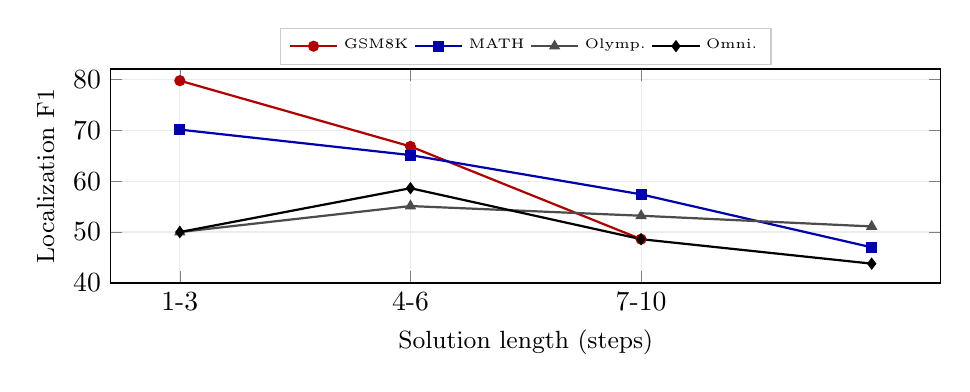
\begin{tikzpicture}
    \begin{axis}[width=\linewidth, height=4.3cm, symbolic x coords={1-3,4-6,7-10,11+}, xtick=data,
      xlabel={Solution length (steps)}, xlabel style={font=\small}, ylabel={Localization F1}, ylabel style={font=\small},
      ymin=40, ymax=82, grid=major, grid style={gray!15},
      legend style={font=\tiny, at={(0.5,1.02)}, anchor=south, legend columns=4, draw=gray!40}]
    \addplot[thick,mark=*,mark size=1.6pt,red!70!black] coordinates {(1-3,79.7)(4-6,66.8)(7-10,48.6)};
    \addplot[thick,mark=square*,mark size=1.6pt,blue!70!black] coordinates {(1-3,70.1)(4-6,65.1)(7-10,57.4)(11+,47.0)};
    \addplot[thick,mark=triangle*,mark size=1.6pt,gray!60!black] coordinates {(1-3,50.0)(4-6,55.1)(7-10,53.2)(11+,51.1)};
    \addplot[thick,mark=diamond*,mark size=1.6pt,black] coordinates {(1-3,50.0)(4-6,58.6)(7-10,48.6)(11+,43.8)};
    \legend{GSM8K,MATH,Olymp.,Omni.}
    \end{axis}
  \end{tikzpicture}
  \subcaption{F1 by solution length.}\label{fig:length}
  \end{subfigure}\hfill
  \begin{subfigure}{0.49\linewidth}\centering
  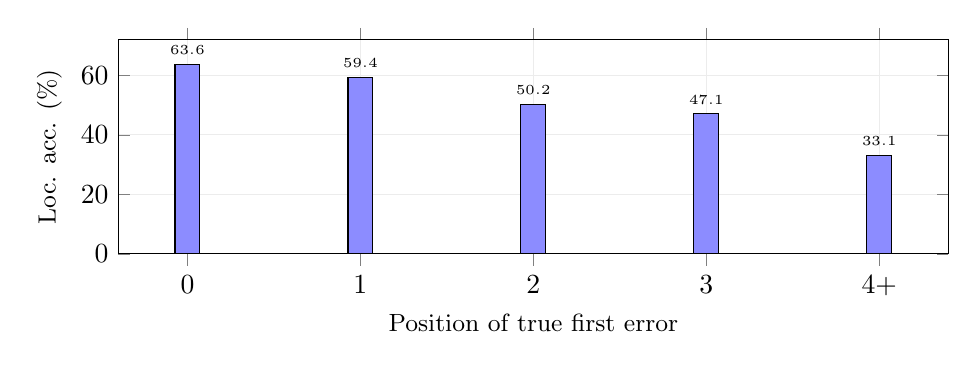
\begin{tikzpicture}
    \begin{axis}[width=\linewidth, height=4.3cm, ybar, bar width=9pt, symbolic x coords={0,1,2,3,4+}, xtick=data,
      xlabel={Position of true first error}, xlabel style={font=\small}, ylabel={Loc. acc. (\%)}, ylabel style={font=\small},
      ymin=0, ymax=72, grid=major, grid style={gray!15},
      nodes near coords, nodes near coords style={font=\tiny}]
    \addplot[fill=blue!45] coordinates {(0,63.6)(1,59.4)(2,50.2)(3,47.1)(4+,33.1)};
    \end{axis}
  \end{tikzpicture}
  \subcaption{Accuracy by error position.}\label{fig:errpos}
  \end{subfigure}
  \caption{Localization for LVH-1.5B degrades with solution length \textbf{(a)} and with a later error position \textbf{(b)}, because the head must first pass every earlier step.}
  \label{fig:lengthpos}
\end{figure}

\subsection{Introspection is complementary to generation}
\label{sec:exp-fusion}

The two signals read different evidence, so we test whether they combine. We form a logit space sum of the introspective reward and a generative verifier score, with a single weight and bias fixed on a held out MATH split and never on the test subsets. On matched 120 case slices of the four subsets, this fixed combination improves the mean localization F1 by 5.4 points over the greedy generative verifier alone. The gain is not a re-ranking of the same errors. The head recovers cases where a fluent but wrong step misleads the surface verdict, and the generative verifier keeps the cases where a written derivation is needed, so the sum is above either input. This is the practical form of the finding: an introspective read is not only cheap, it carries evidence that a generative verifier does not already have.

\subsection{At 7B, generation earns its cost, and introspection remains a near free add on}
\label{sec:exp-7b}

We repeat the study at 7B on 120 case slices in the bottom panel of \Cref{tab:pb}. Here the generative verifier is stronger, 76.8 mean F1, and the introspective head alone no longer matches it. Its raw logits carry a per domain offset at 7B, most visible on OlympiadBench, so we center them per domain with an unsupervised median shift estimated on the domain's own scores, with no labels. This raises the standalone head from 64.2 to 68.5 mean F1 (\Cref{app:calib}), but it is still short of the generative verifier, which marks the regime where generation is worth its cost. The head remains useful as an add on. The honest leave one domain out fusion, which never tunes on the domain it scores, improves MATH and OlympiadBench, does not lower any subset, and raises the mean from 76.8 to 77.4. This per domain centering assumes the test domain is known at inference; a domain agnostic global centering returns only the generative baseline of 76.8, so the gain depends both on this domain metadata and on the calibration itself (\Cref{app:calib}). The picture across scales gives a simple cost accuracy rule. At small scale the introspective head is Pareto optimal, matching or beating trained process reward models from one forward pass (\Cref{fig:pareto}). At large scale it is a near free add on to a generative process reward model, since one extra forward pass is negligible next to repeated decoding.

\Cref{fig:fusion} decomposes the 7B fusion by subset. It matches or beats the generative verifier everywhere and gains where the verifier has room, plus 1.5 on MATH and plus 0.9 on OlympiadBench, while it stays level on the subsets the verifier already handles. The complementarity is also visible case by case. \Cref{fig:agree} classifies the 480 shared cases by which verifier is right. The two agree on the outcome in 342 cases, both correct in 275 and both wrong in 67. Of the 138 where exactly one is right, the generative verifier is right more often, 98 against 40, which is why it is the stronger verifier at 7B, while the 40 cases the head uniquely fixes are what the fusion recovers. \Cref{app:cases} analyzes one case from each cell. The fusion is insensitive to the exact weight it places on the head, with a broad plateau of near optimal weights (\Cref{fig:fusionweight}).

\begin{figure}[t]
  \centering
  \begin{minipage}[b]{0.63\linewidth}\centering
    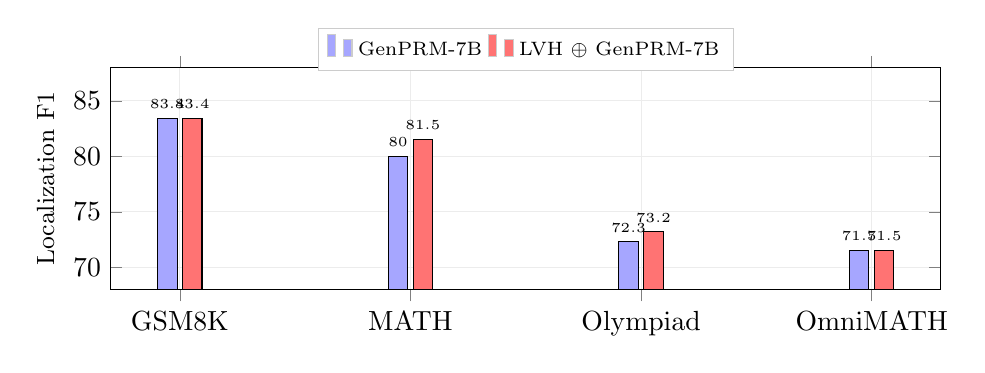
\begin{tikzpicture}
      \begin{axis}[
        width=\linewidth, height=4.4cm,
        ybar, bar width=7pt,
        symbolic x coords={GSM8K, MATH, Olympiad, OmniMATH},
        xtick=data, ymin=68, ymax=88, ylabel={Localization F1}, ylabel style={font=\small},
        legend style={at={(0.5,1.18)}, anchor=north, legend columns=2, font=\scriptsize, draw=gray!40},
        grid=major, grid style={gray!15},
        nodes near coords, nodes near coords style={font=\tiny},
        every node near coord/.append style={/pgf/number format/fixed, /pgf/number format/precision=1},
      ]
      \addplot[fill=blue!35] coordinates {(GSM8K,83.4)(MATH,80.0)(Olympiad,72.3)(OmniMATH,71.5)};
      \addplot[fill=red!55] coordinates {(GSM8K,83.4)(MATH,81.5)(Olympiad,73.2)(OmniMATH,71.5)};
      \legend{GenPRM-7B, LVH $\oplus$ GenPRM-7B}
      \end{axis}
    \end{tikzpicture}
    \subcaption{Fusion decomposition by subset.}\label{fig:fusion}
  \end{minipage}\hfill
  \begin{minipage}[b]{0.34\linewidth}\centering
    \small
    \begin{tabular}{lcc}
      \toprule
      & \multicolumn{2}{c}{Generative} \\
      Head & correct & wrong \\
      \midrule
      correct & 275 & \textbf{40} \\
      wrong   & \textbf{98} & 67 \\
      \bottomrule
    \end{tabular}
    \vspace{2mm}
    \subcaption{Agreement on 480 cases.}\label{fig:agree}
  \end{minipage}
  \caption{Complementarity at 7B. \textbf{(a)} The honest leave one domain out fusion matches or beats the generative verifier on every subset, gaining where it has room. \textbf{(b)} The head uniquely fixes 40 cases the generative verifier gets wrong, which is what the fusion recovers.}
  \label{fig:complement}
\end{figure}

\subsection{Compute accounting}
\label{sec:exp-compute}

The cost gap is the point of the method, so we make it explicit on two axes, token compute and measured wall clock. The introspective head reads the solution once and produces every step reward in that single forward pass, with no autoregressive decoding and no interpreter call. A single greedy pass of the same size generative verifier reads the same solution and then decodes a critique, and it also runs code. On our 7B outputs the critique is about 3.5 times as many tokens as the solution, measured over 480 cases. In token compute, reading is one prefill while decoding is one forward pass per generated token, so a single greedy generative pass costs about four times the token compute of the head, and the head spends about one quarter of it. Wall clock makes the gap larger, because the decoded tokens are produced one forward pass at a time while the head reads all tokens in a single parallel prefill. On one V100 at 7B, the greedy generative verifier takes a median of 31 seconds per solution end to end including code execution, while the introspective head scores the same solution in about 1 second unbatched, a median speedup near 32 times. We compare against the greedy verifier throughout, since sampling and voting would raise the cost of both verifiers. The head therefore sits at a different point on the cost accuracy curve. It reaches a mean F1 in the range of a strong single pass generative verifier while spending the compute of a single read.

\begin{figure}[t]
  \centering
  \begin{minipage}[b]{0.49\linewidth}\centering
    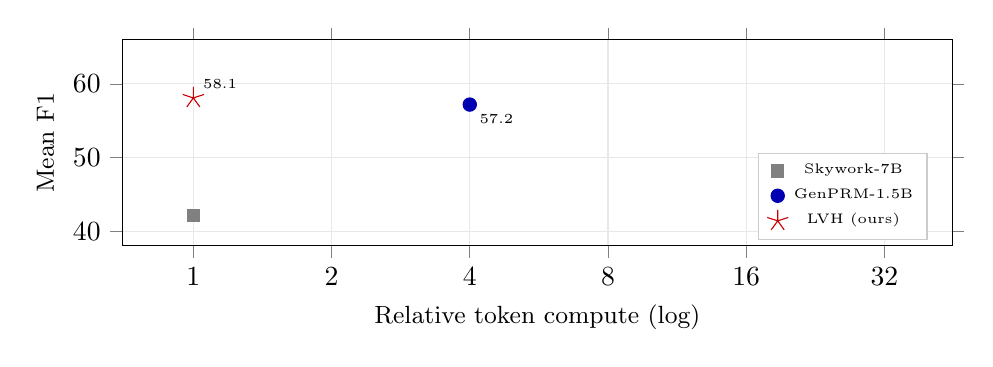
\begin{tikzpicture}
      \begin{axis}[
        width=\linewidth, height=4.2cm,
        xmode=log, log basis x=2,
        xtick={1,2,4,8,16,32}, xticklabels={1,2,4,8,16,32},
        xlabel={Relative token compute (log)}, xlabel style={font=\small},
        ylabel={Mean F1}, ylabel style={font=\small},
        ymin=38, ymax=66, xmin=0.7, xmax=45,
        grid=both, grid style={gray!18}, tick align=outside,
        legend pos=south east, legend style={font=\tiny, fill=white, draw=gray!40},
      ]
      \addplot[only marks, mark=square*, mark size=2.2pt, color=gray] coordinates {(1,42.1)};
      \addlegendentry{Skywork-7B}
      \addplot[only marks, mark=*, mark size=2.4pt, color=blue!70!black] coordinates {(4,57.2)};
      \addlegendentry{GenPRM-1.5B}
      \addplot[only marks, mark=star, mark size=4pt, color=red!80!black] coordinates {(1,58.1)};
      \addlegendentry{LVH (ours)}
      \node[anchor=south west, font=\tiny] at (axis cs:1,58.1) {58.1};
      \node[anchor=north west, font=\tiny] at (axis cs:4,57.2) {57.2};
      \end{axis}
    \end{tikzpicture}
    \subcaption{Cost--accuracy frontier (1.5B).}\label{fig:pareto}
  \end{minipage}\hfill
  \begin{minipage}[b]{0.49\linewidth}\centering
    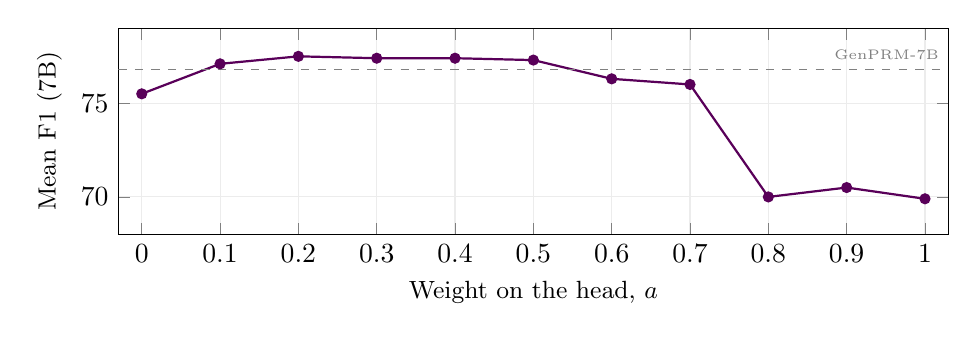
\begin{tikzpicture}
      \begin{axis}[width=\linewidth, height=4.2cm, xlabel={Weight on the head, $a$}, xlabel style={font=\small},
        ylabel={Mean F1 (7B)}, ylabel style={font=\small},
        xmin=-0.03, xmax=1.03, ymin=68, ymax=79, grid=major, grid style={gray!15}]
      \addplot[thick, mark=*, mark size=1.6pt, color=violet!70!black] coordinates {(0,75.5)(0.1,77.1)(0.2,77.5)(0.3,77.4)(0.4,77.4)(0.5,77.3)(0.6,76.3)(0.7,76.0)(0.8,70.0)(0.9,70.5)(1.0,69.9)};
      \draw[dashed,gray] (axis cs:-0.03,76.8)--(axis cs:1.03,76.8);
      \node[anchor=south east,font=\tiny,gray] at (axis cs:1.03,76.8) {GenPRM-7B};
      \end{axis}
    \end{tikzpicture}
    \subcaption{Fusion is robust to the mixing weight.}\label{fig:fusionweight}
  \end{minipage}
  \caption{\textbf{(a)} At 1.5B the introspective head (star) reaches higher mean F1 than a greedy generative pass at about one quarter of its token compute (GPT-4o, 61.9, omitted as a much larger model). \textbf{(b)} The 7B fusion mean F1 against the weight $a$ on the head; a broad plateau spans $a\in[0.1,0.5]$, so the fusion is insensitive to the exact weight.}
  \label{fig:costfusion}
\end{figure}

\subsection{Honest notes}
\label{sec:exp-honest}

The clearest limitation of the cheap head is OmniMATH, the proof heavy subset. Its per step separability is the lowest of the four subsets, a step level AUC of 0.866 (\Cref{tab:perdomain}), and the sharper limit is that the head over flags correct proofs and mislocates errors on long solutions, which is why it is weakest there and why the fusion defers to the generative verifier on it (\Cref{app:omnimath}). The per domain median shift that the 7B fusion uses is a scale specific trick, not a component of the method, and we explain in \Cref{app:calib} why the 7B head needs it and the 1.5B head does not.

% Conclusion for the Introspective Verification paper.
% Style: plain, direct; no em-dashes; minimal colons/quotes; no anthropomorphic verbs.

\section{Conclusion}
\label{sec:conclusion}

We asked whether the judgment that a generative process reward model produces by decoding a critique is already available in the verifier's hidden states, without generation. It is. Step correctness is decodable by a probe on an intermediate layer of the backbone, near seventy percent of the depth, more strongly than from the final layer, because the final state is shaped to emit the surface verdict while an earlier state reflects whether the step follows from its premises. We turned this into an introspective verdict head, a residual readout over an intermediate and a final layer, trained with LoRA on step labels and evaluated in a single forward pass on a single V100. On ProcessBench at 1.5B it reaches 58.1 mean F1, above most trained process reward models including ones at 7B and 14B scale and above a same size generative model, from a read that is about an order of magnitude faster in wall clock than a generative pass. The two signals are complementary, and a fixed combination with a generative verifier improves it at both scales.

The picture we report is deliberately honest about where the cheap read stops. At matched training the residual form does not raise the mean over the strongest single readout; it redistributes accuracy toward the proof heavy subsets while the intermediate view alone is the weaker of the two. The per domain calibration that helps the 7B head hurts the 1.5B head, so we present it as a scale specific trick rather than a component of the method. The head is over confident and needs a tuned threshold, its localization is coarser than an explicit re-derivation on the hardest subsets, and it cannot catch errors of omission, which are invisible to any step local read. These are limits of reading a single forward pass, and they mark the regime where generation earns its cost.

Two directions follow. The first is downstream use, since a verifier is ultimately measured by the answers it selects, and an introspective reward that costs one read is attractive for Best of N selection and for search. The second is to close the localization gap on proof heavy problems, either by reading more than one intermediate layer or by spending a short generation only on the steps where the head is uncertain, which keeps the average cost near one read while recovering the cases where generation currently wins. More broadly, the result suggests that verification, like other judgments a model can make about its own computation, may not need to be spoken to be read.


\bibliography{references}
\bibliographystyle{iclr2027_conference}

\appendix
% Appendix: supporting detail and case studies for Introspective Verification.
% All numbers are computed from the released dumps of our own runs (layerfeats.npz,
% pa15_full.npz, pa_4000_ml4096.npz) with the localization-F1 metric of the main text.
% Style: plain, direct; no em-dashes; minimal colons/quotes.

\section{Supporting detail}
\label{app:experiments}

This appendix collects supporting detail and two case studies. \Cref{app:layersweep} gives the full per layer probe numbers behind \Cref{fig:layersweep}, \Cref{app:calib} explains the scale specific median shift used only at 7B, and \Cref{app:omnimath} documents the OmniMATH ranking limit. The two case studies in \Cref{app:cases} show, on real ProcessBench cases, the complementary failures that the fusion of \Cref{sec:exp-7b} exploits. Unless stated otherwise the metric is ProcessBench localization F1 and every number is computed from our own score dumps.

\subsection{Per layer probe sweep}
\label{app:layersweep}

\Cref{fig:layersweep} plots the per layer probe separability of \Cref{tab:layersweep} as a curve against relative depth. We freeze the 7B backbone, take the last token hidden state of each step at eight candidate layers, fit a balanced logistic probe on step correctness, and report the step level AUC on a held out split of the training pool and the probe localization F1 on 140 held out cases. Both peak at about seventy percent of the depth and fall off toward the final layer and toward the middle of the network.

\begin{figure}[h]
  \centering
  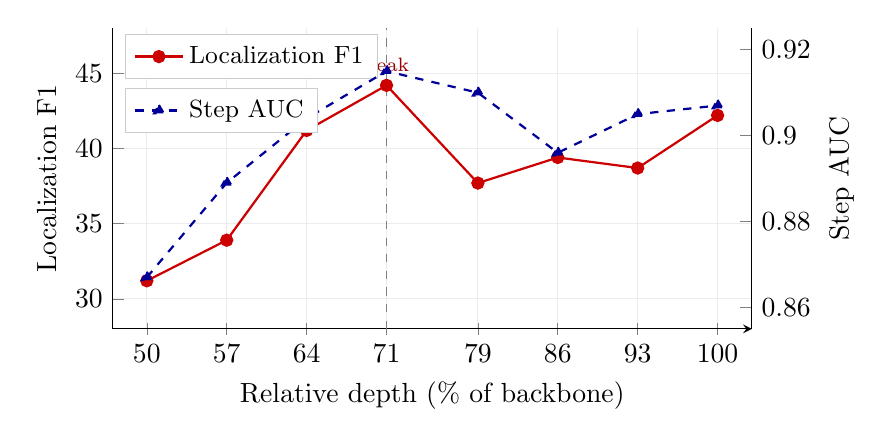
\begin{tikzpicture}
    \begin{axis}[
      width=0.80\linewidth, height=5.4cm,
      axis y line*=left, axis x line=bottom,
      xlabel={Relative depth (\% of backbone)}, ylabel={Localization F1},
      xmin=47, xmax=103, ymin=28, ymax=48,
      xtick={50,57,64,71,79,86,93,100},
      ytick={30,35,40,45},
      grid=major, grid style={gray!15},
      legend style={at={(0.02,0.98)}, anchor=north west, font=\small, draw=gray!40},
    ]
    \addplot[mark=*, thick, color=red!80!black] coordinates {(50,31.2)(57,33.9)(64,41.2)(71,44.2)(79,37.7)(86,39.4)(93,38.7)(100,42.2)};
    \addlegendentry{Localization F1}
    \draw[dashed, gray] (axis cs:71,28) -- (axis cs:71,48);
    \node[anchor=south, font=\scriptsize, red!60!black] at (axis cs:71,44.2) {peak};
    \end{axis}
    \begin{axis}[
      width=0.80\linewidth, height=5.4cm,
      axis y line*=right, axis x line=none,
      ylabel={Step AUC}, ymin=0.855, ymax=0.925,
      xmin=47, xmax=103, ytick={0.86,0.88,0.90,0.92},
      legend style={at={(0.02,0.80)}, anchor=north west, font=\small, draw=gray!40},
    ]
    \addplot[mark=triangle*, thick, dashed, color=blue!60!black] coordinates {(50,0.867)(57,0.889)(64,0.904)(71,0.915)(79,0.910)(86,0.896)(93,0.905)(100,0.907)};
    \addlegendentry{Step AUC}
    \end{axis}
  \end{tikzpicture}
  \caption{Per layer probe separability on the frozen 7B backbone (the curve behind \Cref{tab:layersweep}). Both the step level AUC (right axis) and the probe localization F1 (left axis) peak at about seventy percent of the depth and fall off toward the final layer at the right edge.}
  \label{fig:layersweep}
\end{figure}

\subsection{A calibration trick for the 7B fusion}
\label{app:calib}

The 7B fusion uses one small unsupervised trick, which we report for completeness rather than as part of the method. The 7B head assigns systematically different logit levels to different domains, so a single global decision threshold is misaligned per domain and is too strict on OlympiadBench in particular. Subtracting each domain's own median logit, which needs no labels, realigns the domains to a common threshold. This raises the standalone 7B head from 64.2 to 68.5 mean F1 and is what lets the honest fusion reach 77.4. The 1.5B head does not show this drift. Its per domain logit levels already sit near a common threshold, so the same shift adds nothing and slightly hurts, since on OmniMATH it removes useful spread. The difference is one of scale, the larger and more specialized backbone separates domains more strongly in its logit scale, so we apply the shift only at 7B.

\subsection{The OmniMATH ranking limit}
\label{app:omnimath}

OmniMATH is the proof heavy subset and the hardest for the cheap head. Its per step separability is the lowest of the four subsets, a step level AUC of 0.866 against 0.889 on GSM8K (\Cref{tab:perdomain}), but the sharper limit is localization on correct and on long solutions. The head has its lowest correct solution accuracy on OmniMATH, 57.7 percent, so it over flags correct proofs, and its highest wrong step rate, 44.3 percent, so when a proof is wrong it often marks the wrong step. Both effects grow with solution length (\Cref{fig:length,fig:errpos}). This is why the standalone head is weakest on OmniMATH in \Cref{tab:pb}, and why the fusion defers to the generative verifier there. We treat it as an honest limit of a single forward pass read on long free form proofs.

\section{Extended quantitative analysis}
\label{app:extended}

We analyze the head in more depth from the same score dumps. Unless noted the scale is 1.5B on the full benchmark, and the metric is localization F1 or step level AUC as defined in \Cref{sec:exp-setup}.

\subsection{Threshold sensitivity}
\label{app:thr}

The head returns a per step probability, and a single threshold turns it into a decision. \Cref{fig:thrsweep} sweeps this threshold per subset. GSM8K is nearly flat and peaks around 0.87, while the proof heavy subsets keep improving toward a stricter threshold, since the head over flags there and a higher bar removes false alarms. A single threshold tuned on a held out split, 0.92, is a compromise across subsets. This per subset disagreement in the best threshold is what the unsupervised per domain calibration of \Cref{app:calib} exploits at 7B.

\begin{figure}[h]
  \centering
  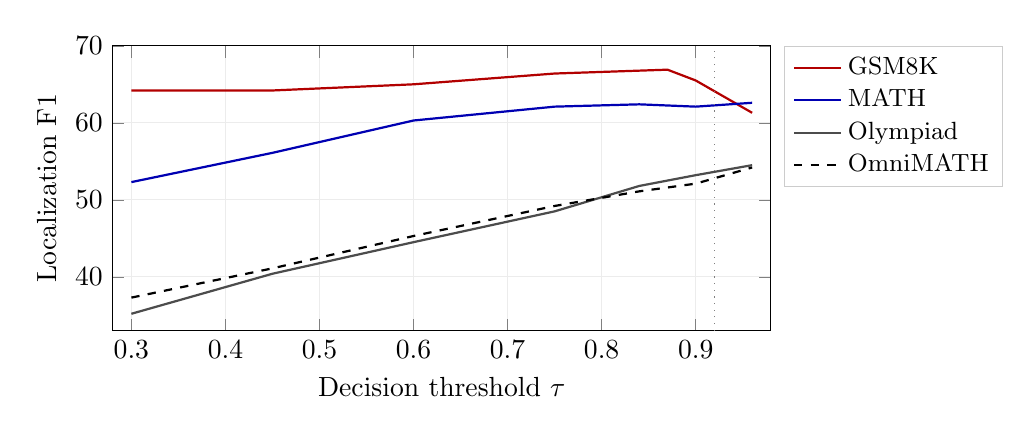
\begin{tikzpicture}
    \begin{axis}[width=0.82\linewidth, height=5.2cm, xlabel={Decision threshold $\tau$}, ylabel={Localization F1},
      xmin=0.28, xmax=0.98, ymin=33, ymax=70, grid=major, grid style={gray!15},
      legend style={at={(1.02,1)}, anchor=north west, font=\small, draw=gray!40}, legend cell align=left]
    \addplot[thick,color=red!70!black] coordinates {(0.3,64.2)(0.45,64.2)(0.6,65.0)(0.75,66.4)(0.87,66.9)(0.9,65.5)(0.96,61.3)};
    \addlegendentry{GSM8K}
    \addplot[thick,color=blue!70!black] coordinates {(0.3,52.3)(0.45,56.1)(0.6,60.3)(0.75,62.1)(0.84,62.4)(0.9,62.1)(0.96,62.6)};
    \addlegendentry{MATH}
    \addplot[thick,color=gray!60!black] coordinates {(0.3,35.2)(0.45,40.4)(0.6,44.5)(0.75,48.5)(0.84,51.8)(0.9,53.2)(0.96,54.5)};
    \addlegendentry{Olympiad}
    \addplot[thick,dashed,color=black] coordinates {(0.3,37.3)(0.45,41.1)(0.6,45.3)(0.75,49.2)(0.84,51.1)(0.9,52.1)(0.96,54.2)};
    \addlegendentry{OmniMATH}
    \draw[dotted,gray] (axis cs:0.92,33)--(axis cs:0.92,70);
    \end{axis}
  \end{tikzpicture}
  \caption{Localization F1 against the decision threshold for LVH-1.5B. GSM8K peaks early while the proof heavy subsets prefer a stricter threshold. The dotted line is the single held out tuned threshold.}
  \label{fig:thrsweep}
\end{figure}

\subsection{Calibration}
\label{app:calibration}

The head returns a probability, and \Cref{fig:calib} checks how well that probability matches the empirical error rate. It does not. The head is over confident, with an expected calibration error of 0.238, and steps to which it assigns a probability near one are in fact error steps only 41 percent of the time. This is why inference tunes a single threshold rather than reading the probability at 0.5, and it is consistent with the per domain offset that the 7B head shows in \Cref{app:calib}. The ranking is still useful, as the high step level AUC in \Cref{tab:perdomain} shows, but the raw probability should not be read as a calibrated confidence.

\begin{figure}[h]
  \centering
  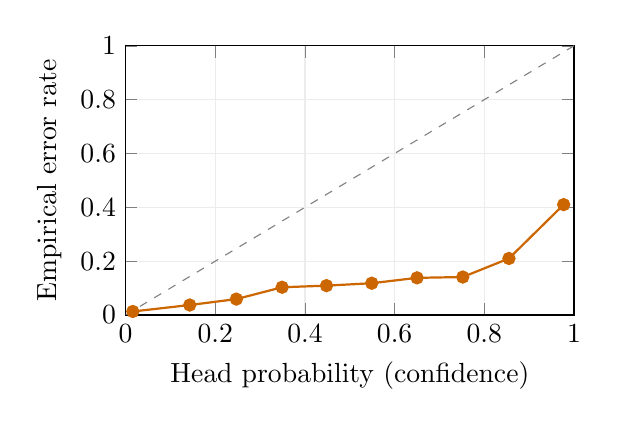
\begin{tikzpicture}
    \begin{axis}[width=0.6\linewidth, height=5.0cm, xlabel={Head probability (confidence)}, ylabel={Empirical error rate},
      xmin=0, xmax=1, ymin=0, ymax=1, grid=major, grid style={gray!15}]
    \addplot[dashed,gray] coordinates {(0,0)(1,1)};
    \addplot[thick,mark=*,color=orange!80!black] coordinates {(0.016,0.013)(0.143,0.037)(0.247,0.059)(0.349,0.103)(0.448,0.109)(0.549,0.118)(0.65,0.138)(0.752,0.141)(0.855,0.21)(0.977,0.41)};
    \end{axis}
  \end{tikzpicture}
  \caption{Reliability of LVH-1.5B. The head is over confident, the curve sits well below the diagonal, so a high score does not mean a high error probability (ECE $=0.238$).}
  \label{fig:calib}
\end{figure}

\section{Case analysis}
\label{app:cases}

We walk through four real ProcessBench cases at 7B, one for each cell of \Cref{fig:agree}. Each box shows the problem and its solution steps, with a mark for whether the generative verifier (\textbf{Gen}) and the introspective head (\textbf{Head}) judge the step correct (\vgood) or an error (\vbad). The step highlighted in the text is the labeled first error. The generative verifier marks a step an error when its value drops below one half; the head marks a step an error when its probability exceeds its 7B operating threshold, about 0.75.

\begin{tcolorbox}[breakable, colback=gray!2, colframe=gray!55, fonttitle=\bfseries\small,
  title={Case 1 (GSM8K). The head catches a fluent but wrong step that generation accepts.}, boxrule=0.5pt, left=2mm, right=2mm, top=1mm, bottom=1mm]
\footnotesize
\textbf{Problem.} It takes James 10 minutes to read 3 pages before bed. He reads 18 pages, then goes to sleep. How long does James spend reading? \emph{(Correct: $18 \div 0.3 = 60$ minutes.)}
\smallskip
\begin{tabularx}{\linewidth}{@{}c X c c@{}}
\toprule
\# & Step & Gen & Head \\
\midrule
1 & Set up: find a reading rate, then use it & \vgood & \vgood \\
2 & Rate $= 3/10 = 0.3$ pages per minute & \vgood & \vgood \\
3 & Total pages read $= 18$ & \vgood & \vgood \\
4 & \textbf{Time $= 18 \times 0.3 = 5.4$ minutes} \; \emph{(first error: needs $\div$, not $\times$)} & \vgood & \vbad \\
5 & Answer: $5.4$ minutes & \vgood & \vbad \\
\bottomrule
\end{tabularx}
\smallskip

\textbf{Gold:} step 4. \quad \textbf{Gen predicts:} none (misses the error). \quad \textbf{Head predicts:} \textbf{step 4 (correct)}.
\smallskip

\textbf{Why.} The two readouts diverge here. The final layer state follows the surface form of the step, and $18 \times 0.3 = 5.4$ is a fluent, locally valid multiplication, so the generated verdict accepts it. The intermediate layer encodes the step against its premises, where the rate is pages per minute and the question asks for minutes, so the correct operation is division; that mismatch is present in the intermediate representation before the surface token is formed, and the residual head reads it out. This is the paper's mechanism in one example, the latent assessment catches a reasoning error that the stated verdict does not.
\end{tcolorbox}

\begin{tcolorbox}[breakable, colback=gray!2, colframe=gray!55, fonttitle=\bfseries\small,
  title={Case 2 (GSM8K). The head avoids a false alarm that generation raises on a correct solution.}, boxrule=0.5pt, left=2mm, right=2mm, top=1mm, bottom=1mm]
\footnotesize
\textbf{Problem.} A two hour concert gives each group 2 minutes on, 6 to perform, 2 off, plus one 10 minute intermission. How many groups can perform? \emph{(Correct: $10n+10\le 120 \Rightarrow 11$ groups; every step is correct.)}
\smallskip
\begin{tabularx}{\linewidth}{@{}c X c c@{}}
\toprule
\# & Step & Gen & Head \\
\midrule
1 & Fit group slots into 120 minutes & \vgood & \vgood \\
2 & Per group $2+6+2 = 10$ minutes \; \emph{(correct)} & \vbad & \vgood \\
3 & Add the 10 minute intermission & \vbad & \vgood \\
4 & Total for $n$ groups is $10n+10$ & \vbad & \vgood \\
5 & Solve $10n+10 \le 120$ & \vbad & \vgood \\
6 & $n \le 11$ & \vbad & \vgood \\
7 & Answer: 11 groups & \vbad & \vgood \\
\bottomrule
\end{tabularx}
\smallskip

\textbf{Gold:} none. \quad \textbf{Gen predicts:} step 2 (false alarm). \quad \textbf{Head predicts:} \textbf{none (correct)}.
\smallskip

\textbf{Why.} The generative verifier reaches its verdict by re-deriving the step, and its own derivation for the per group time disagrees with the solution, so it reports an error where there is none. The head does not re-derive. It reads whether the step is consistent with its premises, and $2+6+2=10$ is, so its error probability stays low on every step. The head is less exposed to this self-inflicted false alarm because it does not run a second, fallible generation. This is the complementary win to Case 1, and the reason the two signals combine well (\Cref{sec:exp-7b}).
\end{tcolorbox}

\begin{tcolorbox}[breakable, colback=gray!2, colframe=gray!55, fonttitle=\bfseries\small,
  title={Case 3 (MATH). Generation localizes an error that the head places one step too early.}, boxrule=0.5pt, left=2mm, right=2mm, top=1mm, bottom=1mm]
\footnotesize
\textbf{Problem.} Let $x>0$ satisfy $x - \tfrac{1}{x} = 3$. Find $x + \tfrac{1}{x}$. \emph{(Correct: $x+\tfrac1x=\sqrt{13}$.)}
\smallskip
\begin{tabularx}{\linewidth}{@{}c X c c@{}}
\toprule
\# & Step & Gen & Head \\
\midrule
1 & $x^2 = 3x + 1$ \; \emph{(correct)} & \vgood & \vbad \\
2 & \textbf{$x^2 - 3x = 1$, factor $(x-1)(x-3)=0$} \; \emph{(first error: wrong factoring)} & \vbad & \vbad \\
3 & $x = 3$, so $x + 1/x = 10/3$ & \vbad & \vbad \\
4 & Answer: $4$ & \vbad & \vbad \\
\bottomrule
\end{tabularx}
\smallskip

\textbf{Gold:} step 2. \quad \textbf{Gen predicts:} \textbf{step 2 (correct)}. \quad \textbf{Head predicts:} step 1 (one step early).
\smallskip

\textbf{Why.} The head localizes to the region of the error but not the exact step. Its per step probability already saturates at step one, the correct setup that leads straight into the bad factoring, so it fires one step early. The intermediate signal is coarse in position, it marks that the derivation is heading wrong, while the fine boundary between the correct setup and the incorrect factoring is exactly what an explicit step by step re-derivation resolves. The generative verifier performs that re-derivation and pins step two. This coarser localization is the price of a single read, and it is why generation still wins the harder localizations at 7B (\Cref{fig:agree}).
\end{tcolorbox}

\begin{tcolorbox}[breakable, colback=gray!2, colframe=gray!55, fonttitle=\bfseries\small,
  title={Case 4 (GSM8K). Both verifiers miss an omission at the first step.}, boxrule=0.5pt, left=2mm, right=2mm, top=1mm, bottom=1mm]
\footnotesize
\textbf{Problem.} In a family of 5, three people eat three eggs each day and the other two eat two each. How many eggs in a week? \emph{(Correct: $(3\cdot3 + 2\cdot2)\cdot7 = 91$.)}
\smallskip
\begin{tabularx}{\linewidth}{@{}c X c c@{}}
\toprule
\# & Step & Gen & Head \\
\midrule
1 & \textbf{Count $3$ people $\times 3$ eggs, then $\times 7$ days} \; \emph{(first error: omits the other 2 people)} & \vgood & \vgood \\
2 & $9$ eggs/day $\times 7 = 63$ & \vbad & \vgood \\
3 & $63$ eggs & \vbad & \vbad \\
\bottomrule
\end{tabularx}
\smallskip

\textbf{Gold:} step 1. \quad \textbf{Gen predicts:} step 2 (wrong). \quad \textbf{Head predicts:} step 3 (wrong).
\smallskip

\textbf{Why.} The error is one of omission, not of a wrong statement. Step one, count three people times three eggs, is true as far as it goes; what is wrong is the missing contribution of the other two people, which never appears as a locally incorrect step. Both verifiers score each step against its premises, and a step that is locally valid but incomplete passes either test, so both drift to a later step. Errors of omission are a property of the whole solution rather than of one step, so a step local read, generative or introspective, shares this blind spot. These are the 67 both wrong cases of \Cref{fig:agree}, and they mark where step level verification itself, not the choice of reading it, reaches its limit.
\end{tcolorbox}


\end{document}
